\chapter{Theoretical Foundations}\label{ch:theoretical-foundations}


\section{Sheet Metal}\label{sec:sheet-metal}
% Definition
Sheet metal is usually manufactured by flat rolling any type of metal and thus characterized by
its aspect ratio of thickness and surface area typically ranging from 0.4 mm to 6mm.
Above this range, its is considered to be a plate and below it is considered to be
foil~\cite[p. 405]{groover_fundamentalsmodernmanufacturing_2020}.
% Material
Low-carbon steel is the most commonly used type of sheet metal because it is low cost and has a good form ability as
well as its sufficient strength for most applications~\cite[p. 405]{groover_fundamentalsmodernmanufacturing_2020}.
% Commercial importance
Sheet metals play a vital role in many industries most notably automotive and aerospace to reduce the weight of
products~\cite[pp. 1]{zheng_reviewformingtechniques_2018}.

\subsection*{Sheet Metal Manufacturing}
% Manufacturing methods
Sheet metal working is primarily carried out using machine tools known as presses and the process
is referred to as sheet-metal press-working.
To carry out this processes stamping presses are used which are equipped with punch and die
tooling which is specifically designed for this purpose
\cite[p. 405]{groover_fundamentalsmodernmanufacturing_2020}.
The punch is a shaped tool that is usually mounted as upper part on the press ram and applies
pressure on the sheet metal to shape it.
The die is a stationary tool that is mounted in the press bed and provides a support surface for
the sheet metal and also defines the shape of the finished
product~\ref{sec:bending}~\cite[p. 412]{groover_fundamentalsmodernmanufacturing_2020}.

While the term "punch" is quite intuitive, the term ``die'' can cause confusion.
The term "die" is typically used to refer to the lower or stationary part of a tooling setup and traces
back to the early days of metal working.
It originated from old English word "dēag" which means a mold, shape, or form most likely refers to the fact that
the metal placed on the die is pressed or molded into a specific shape.

The sheet metal forming processes can be classified into three main categories:
cutting, bending, and drawing.
The process of cutting is employed to divide large sheets of material into smaller pieces while bending and drawing
techniques are employed to shape sheet metal into the desired forms required for creating specific parts.
Bending and drawing are employed to shape sheet metal parts
into their required forms~\cite[p. 405]{groover_fundamentalsmodernmanufacturing_2020}.

The bending bending method used in this study (Air Bending) deploys a mixture of bending and drawing and will be
explained in more detail in the next section.


\section{Sheet Metal Bending}\label{sec:bending}
% Bending definition and description
Bending is a forming operation that is used to change the shape of a sheet metal by
apply a load to it.
It involves using force to shape the sheet mal in into a desired form~\cite[p. 1]{dib_singleensembleclassifiers_2020}.
The load is applied in way that exceeds the yield strength of the metal, but is below its
ultimate tensile strength, which allows the metal to bet permanently deformed into a
new shape~\cite[p. 1]{baig_machinelearningprediction_2021}.
Sheet metal bending is usually used to produce large quantities of components at low cost in various
industries~\cite[p. 1]{dib_singleensembleclassifiers_2020}

During the bending process, the metal sheet undergoes plastic deformation, where the outer fibers are stretches while
the inner fibers are compressed.
This results in a curvature of the sheet metal in the direction of the applied
load~\cite[p. 3]{baig_machinelearningprediction_2021}.
The bending process creates a neutral plane, which an imaginary surface within the metal sheet where there is
neither compression nor stretching. It is also called neutral axis or neutral
line~\cite[pp. 67]{gustafson1998analytical}.
Figure~\ref{fig:neutral-plane} shows the neutral plane after the bending operation, it is
visible, that it is closer to the inside of the bend than to the outside of the bend.
The arrows show where the metal was stretched and where it was compressed.

% Pado:  Since you are including figures, make sure to mention/describe them in the
% text (this
% would be a great opportunity here to define what the punch and die are in this case -
% the
% common meaning of die is „Würfel“ as in „roll the dice“, so the term needs defining
% here for
% the computer science public.

\begin{figure}[h]
    \begin{tcolorbox}[arc=0pt,boxrule=0.5pt, colback=white]
        \centering
        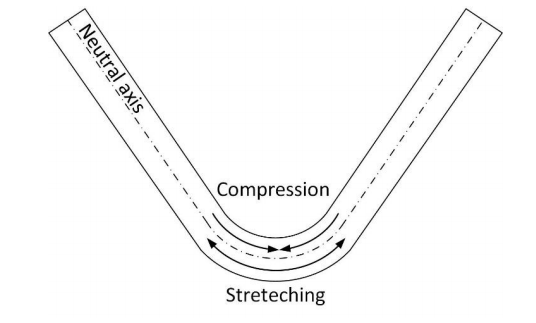
\includegraphics[width=0.6\textwidth]{chap2/images/neutral-plane}
    \end{tcolorbox}
    \caption{Bending plane, compression and stretching of sheet
    metal~\cite[p. 3]{baig_machinelearningprediction_2021}}
    \label{fig:neutral-plane}
\end{figure}

% How curvature is achieved 
The amount of curvature that is achieved in the bending process is determined by the
amount of load applied, the thickness and properties of the metal, and the location and length of the neutral plane.
By controlling these factors, it is possible to achieve precise and consistent results in the bending of sheet metal.

\subsection{Air Bending}\label{subsec:air-bending}
% Definition
Air bending is a variant in the V-Bending process which is performed using puch-and-die
tooling
\cite[p. 416]{groover_fundamentalsmodernmanufacturing_2020}.
In Figure~\ref{fig:air-bending} the air bending process is illustrated.
It can be seen that the punch is mounted on the upper part and applies force on the
sheet metal.
The sheet metal is placed on the die which is mounted on the lower part of the press.


The difference between air- and V-bending is the way the sheet metal is pressed into the die.
Figure~\ref{fig:v-bending} shows the V-bending process, where the sheet metal is pressed into the for of the die.
This process is often used to create complex and precise bends. The die can have different shapes and does not always
have to be a V-shape.
It can also be a U-shape, a Z-shape, or any other shape that is required to achieve the desired bend.
On the other hand, in air bending shown in figure~\ref{fig:air-bending}, the die is open and the sheet metal is not
pressed into the die.
Instead, it bent by applying force to the top of the metal sheet.
The process allows for a wider range of bend angles, as the punch travel distance is not limited by the die.
Additionally, air bending can achive a tighter bend radius compared to V-bending, but may result in a slightly
rounded bed.

Sheet metal bending is a fundamental process in the manufacturing industry, allowing for the creation of various
metal shapes and configurations. Two common techniques are air bending and V-bending, each with unique characteristics.

The primary distinction between air bending and V-bending is the way the sheet metal is pressed into the die. In
V-bending, as illustrated in Figure~\ref{fig:v-bending}, the sheet metal is pressed into the form of the die.
Depending on the die this can produce shapr and precise bends.
The die can have various shapes, including U-shape, Z-shape, or any other shape needed to achieve the desired bend.

In contrast, in air bending, as demonstrated in Figure~\ref{fig:air-bending}, the die is open, and the sheet metal is
not pressed into the die.
Instead, force is applied to the top of the metal sheet, bending it into shape.
This process enables a broader range of bend angles, as the punch travel distance is not restricted by the die.

While air bending can achieve tighter bend radii than V-bending, it may result in a slightly rounded bend. The choice
between air bending and V-bending depends on the specific needs of the manufacturing process.

\begin{figure}[h]
    \begin{tcolorbox}[arc=0pt,boxrule=0.5pt, colback=white]
        \centering
        \begin{subfigure}{0.4\textwidth}
            \centering
            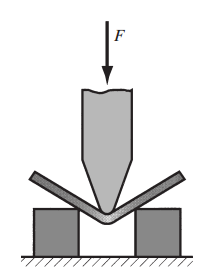
\includegraphics[width=\textwidth]{chap3/images/air-bending}
            \caption{Air bending}
            \label{fig:air-bending}
        \end{subfigure}
        \hfill
        \begin{subfigure}{0.4\textwidth}
            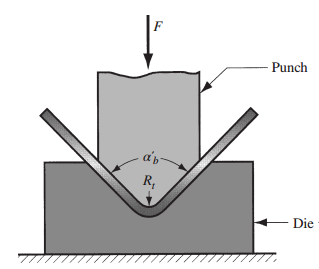
\includegraphics[width=\textwidth]{chap3/images/v-bending}
            \caption{V-Bending}
            \label{fig:v-bending}
        \end{subfigure}
        \hfill
    \end{tcolorbox}
    \caption{Differnt bending methods~\cite[pp. 416]{groover_fundamentalsmodernmanufacturing_2020}}
    \label{fig:bending-methods}
\end{figure}

% Usage of air bending
Air bending is commonly used in automotive industry to manufacture sheet metal
parts~\cite[p. 342]{kim_predictionbendallowance_2007}.
It is typically the preferred bending method because, its high flexibility because it
is possible to achieve different bending angles using the same punch-and-die
tooling~\cite[p. 3]{miranda_formingspringbackprediction_2018}\cite[p. 1]{cruz_applicationmachinelearning_2021}

% Pado: What’s a press brake bending machine?
Today press machines are usually equipped with ``copmputer numeral control (CNC) systems that can automatically
control the bending process and
produce the desired shape''~\cite[p. 3]{miranda_formingspringbackprediction_2018}
The process parameters and their are explained in the section~\ref{sec:process-parameters}.

\subsubsection{Spring Back}\label{sec:spring-back}
% How the spring back is created
When the punch and therefore the bending pressure is removed at the end of the deformation
operation, elastic energy remains in the bent part. This elastic energy is released,
and the
metal sheet partially returns to its original shape. \cite[p.
113-114]{groover_fundamentalsmodernmanufacturing_2020} In metal forming this process is
called
spring back and is illustrated in Figure~\ref{fig:spring-back}.
% Descriptoin of figure 
The solid line shows the metal plate in its original for when the punch was still
applied. The
dashed line shows the metal plate after the punch was removed. The metal plate is
partially
returned to its original shape. The angle before the spring back is usually denoted as $\alpha_f$
and the angle after spring back as $\alpha_i$.
% Introduce of formula
The spring back ($\Delta \alpha_{SB}$) is therefore the difference between $\alpha_f$ and
$\alpha_i$ as show in equation~\ref*{eq:calculation_springback}. \cite[p.
6]{cruz_applicationmachinelearning_2021}

\begin{equation}
    \delta \alpha_{SB} = \alpha_i - \alpha_f
    \label{eq:calculation_springback}
\end{equation}

% Prevent spring back 
To address this issue there are several methods to compensate the spring back. For
example one
common method is over bending, which means that the punch angle and radius are
fabricated smaller
than the specified angle.
\cite[p. 114]{groover_fundamentalsmodernmanufacturing_2020}
Prerequisite for all compensation methods is that the spring back is known therefore
the accurate
prediction of the spring back play an important role in the manufacturing process.

\begin{figure}[h]
    \centering
    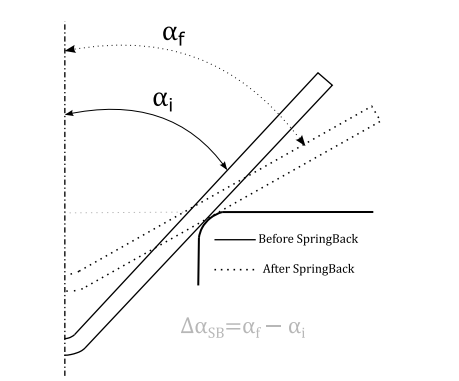
\includegraphics[width=0.5\textwidth]{spring-back}
    \caption{Spring back \cite[p. 5]{cruz_applicationmachinelearning_2021}}
    \label{fig:spring-back}
\end{figure}


\section{Machine Learning}\label{sec:machine-learning}
Machine learning also called \ac{ML} is a field of study that involves using
statistical and
computational techniques to analyze and learn from data. \cite[p.
1]{muller_introductionmachinelearning_2016}

\subsection{Supervised Learning}\label{subsec:supervised-learning}
Supervised learning is a type of machine learning where we have a set of input/output
pairs that
we use to train a model to predict an outcome for a given input. We use this model to make
predictions on new, unseen data, the training set. It consists of the input/output
pairs, needs
to be created manually, but once the model is trained, it can automate and potentially
improve
upon tasks that would be time-consuming or difficult for humans to perform. \cite[p.
25]{muller_introductionmachinelearning_2016}

\subsection{Regression}\label{subsec:regression}
There are two main types of supervised machine learning problems: classification and
regression.
For regression problems it is the goal to predict a continuous numerical value. This
can be a
real number in mathematical terms or a floating-point number in programming terms.
\cite[p. 226]{muller_introductionmachinelearning_2016}
Classification problems involve predicting a class label, which is a choice from a
predefined
list of possible options. \cite[p. 25]{muller_introductionmachinelearning_2016}

Predicting the spring back is a regression problem because the spring back is a
continuous-valued
output.
Therefore, this work focuses on supervised learning for a regression problem and does
not further
consider classification problems.

\subsection{Overfitting and Underfitting}\label{subsec:overfitting-and-underfitting}
% Generalization
In supervised learning, the goal is to construct a model using training data that can
accurately
predict outcomes for new, unseen data that shares similar characteristics as the
training data.
The ability of a model to make accurate predictions on unseen data is referred to as
generalization. The objective is to develop a model that generalizes as effectively as
possible.
\cite[p. 35]{muller_introductionmachinelearning_2016}

The effectiveness of an algorithm on new data is determined by its performance on a
test set.
Simple models tend to generalize better to new data. Overfitting occurs when a model is
too
complex for the amount of information available and does not generalize well, while
underfitting
occurs when a model is too simple and does not perform well on the training set. The
goal is to
find the simplest model that captures the variability in the data.
\cite[p. 35]{muller_introductionmachinelearning_2016}

\subsection{Bias-Variance Tradeoff}\label{subsec:bias-variance-tradeoff}
% Bias 
Bias measures how well the central tendency of a learner's model approximates the
actual function
it is trying to learn. If the model consistently learns the true function accurately,
it is
unbiased. Otherwise, it is biased. \cite[p. 7-8]{neal_biasvariancetradeofftextbooks_2019}
In essence the bias is the differences between the predicted values by the model and
the actual
values.
A high bias indiactes a model with a complex fit to the training data and therefore
overfits
\cite[p. 20]{neal_biasvariancetradeofftextbooks_2019}

% Variance 
Variance measure how much the model's prediction vary, when trained on different
subsets of the
data. That means that a model with low variance generalizes one new data. A high variance
indicates that the model as a complex fit to the data and therefore is overfitting the
training
data. This means it will not perform well on new data. \cite[p.
7-8]{neal_biasvariancetradeofftextbooks_2019}

% Tradeoff 
Both, high variance and high bias are undesirable properties for a model. The goal is,
to find a
model with low bias and low variance. This is called the bias-variance trade off. \cite[p.
9]{neal_biasvariancetradeofftextbooks_2019}

% Regularization
\subsubsection*{Regularization}
Regularization refers to a group of techniques that force a model to be simpler.
this usually results in a slight increase in bias but a substantial decrease in
variance~\cite[p.
12]{burkov2019hundred}.

The regularization method used in this thesis and in general the most popular are L1
and L2
regularization.
In order to construct a regularized model, the objective function is altered by
including a
penalizing term that increases the value as the model becomes more complex~\cite[p.
12]{burkov2019hundred}

\subsection{Ensemble Learning}\label{subsec:ensemble-learning}
Ensemble techniques in machine learning to involve the construction of multiple models
, called
"learners," for a given task. The primary goal of these methods is to improve the
accuracy and
performance of the model by combining the predictions of multiple learners. Ensemble
techniques
differ from single classifier methods by constructing multiple models and combining
them using a
voting strategy in order to highlight different aspects of the data. This can
potentially lead to
improved overall performance. \cite[p. 253]{shaik_briefsurveyrandom_2019}

\subsection{Evaluations and Improvements of Models}

\subsubsection{Cross Validation}
Cross-validation is a method of evaluating the performance of a model by training
multiple models
on different subsets of the data and evaluating their performance. The most common
version of
cross-validation is k-fold cross-validation, in which the data is divided into k folds
, and k
models are trained, each using a different fold as the test set and the remaining folds
as the
training set.
The accuracy of each model is then evaluated, and the average accuracy across all k
models is
used as an estimate of the generalization performance of the model. This process helps
to reduce
the variability in model performance due to the specific choice of training and test
sets, and is
therefore considered to be a more stable and reliable way to evaluate the performance
of a model.
\cite[p. 252-260]{muller_introductionmachinelearning_2016}

\subsubsection{Grid Search}
Each machine learning method has a number of parameters that can be tuned to improve the
performance of the model. Parameters are often not known in advance and must be tuned
to the data.
This is a common task in machine learning and therefore there are standard methods like
grid
search to find the best parameters.
Grid search is a method of systematically working through multiple combinations of
parameters
(called grid), cross-validating as it goes to determine which tune gives the best
performance.
\cite[p. 260-275]{muller_introductionmachinelearning_2016}


\section{State of research}\label{sec:state-of-research}
In recent years, there has been a growing adoption of \ac{ML} in various applications
related to sheet metal forming. With goal to achieve optimal manufacturing quality.
Three main types of \ac{ML} algorithms are used in sheet metal forming applications,
namely supervised learning, unsupervised learning, and reinforcement learning~
\cite[p. 2]{cruz_applicationmachinelearning_2021}.

Sheet metals have a high ratio of yields strength to elastic modulus, which results in
significant spring back, which can compromise the accuracy of the final product.
As a result, extensive research has been carried to estimate the spring back behavior
in sheet metal forming processes~\cite[p. 565]{liu2021deep}.

Current research on mitigating the spring back in sheet metal forming is primarily
focused on compensations methods through numerical simulations, most notably finite
element analysis (FEA)~\cite[p. 565]{liu2021deep}
\cite{lingbeek2005development}  present two methods for compensating spring back in the
deep drawing process, but more reliable simulations is needed of industrial applications.

Also traditional supervised learning methods where used in metal forming applications.

Liu et al. used a \ac{SVM} to predict the spring back in a micro W-bending process,
demonstratring high prediciotn accuracy and generalization performance in comparison to
experimental results~\cite[p. 1]{liu_springbackpredictionforming_2019}
Dib et al. evaluated several \ac{ML} algorithms for predicting the spring back in a
maximum thinning in U-channel and square cup forming processes. The \ac{MLP} found to
be the best model~\cite{dib_singleensembleclassifiers_2020}.
Similarly Abdessalem et al. compared the performance of a quadratic response surface
metod (RSM) and two \ac{SVM} models for determinig the best surrogate model for
probalistic strucutre oprimization of hydrofomred sheet metals. Both \ac{SVM} models
outperformed the RSM model~\cite[]{abdessalem2015probabilistic}.

It has to be noted that most of the research including \ac{ML} relies on FEA to
generate the data for training and testing the models.
This is due to the fact that it is time consuming to obtain enough experimental data for
sheet metal forming processes.
\cite{dib_singleensembleclassifiers_2020} not that the implementations of virtual
tryout still heavily relies on human expertise to make critical decisions.
Also the use of FEM does not necessarily eliminated unexpected defects due to variations
in material properties, tool geometry and process parameters~\cite[p. 2]{
    dib_singleensembleclassifiers_2020}.

% The authors of [21] used SVM to estimate the springback of a micro W-bending process
% with high
% prediction accuracy and generalization performance. The authors of [22] compared the
% performance of different machine learning algorithms (multilayer perceptron type ANN,
% random
% forest, decision tree, naive Bayes, SVM, KNN, and logistic regression) in predicting
% springback
% and maximum thinning in two different forming geometries, namely U-channel and square
% cup. The
% authors concluded that the multilayer perceptron algorithm was the best in
% identifying the
% springback, with a slightly higher score than SVM.
% \cite{cruz_applicationmachinelearning_2021}


% "The literature review shows that FEM methods and Machine Learning approaches are the
% two
% techniques that are vastly applied to predict the springback in sheet metals. Since
% FEM is slow
% so it cannot be used as an on-line tool in the production line for predicting
% springback [29].
% In machine learning, most of the earlier attempts used artificial neural networks
% (ANN) to
% predict springback, which has several limitations. Using ANN, the predictions cannot be
% justified easily, i.e., the explainability of the answer from the neural network is
% very low.
% Neural networks require a lot of computation power to train the model. A neural
% network needs a
% large amount of data so that the model trained is generalized, rather than overfitted
% or under
% fitted to the data."
% \cite{baig_machinelearningprediction_2021}

% "Hence, this research article used tree-based learning algorithms which have high
% explainability, needs less computational power, and need less data to train the model."
% \cite{baig_machinelearningprediction_2021}


% Pado: Expand this discussion a little and move it up (see comment above) 


% There is a considerable amount of literature on modeling of the
% air-bending process. Several significant references are summa-
% rized here briefly. \cite[]{kim_predictionbendallowance_2007}

% Cruz 
With the availability of data there has been an increased use of Machine Learning \ac{
    ML} in
sheet metal forming with the goal to reduce costs and increase manufacturing quality.
\cite{bock_reviewapplicationmachine_2019} \cite[]{cao_manufacturingadvancedsmart_2019}
% Quellen
lesen
The ML algorithms can be divided into the main categories supervised learning,
unsupervised
learning and reinforcement learning. \cite[]{liu_reinforcementlearningfreeform_2020}
Supervised learning is generally used in classification problems and regression
problems while
unsupervised learning is used to find patterns in data \cite[p.
2]{cruz_applicationmachinelearning_2021}.

\subsubsection*{Spring Back Prediction Using Unsupervised Learning}
Artificial Neural Networks \ac{ANN}s are widely used in sheet metal forming because of
their high
accuracy and generalization performance. \cite[p. 2]{cruz_applicationmachinelearning_2021}
\cite[]{narayanasamy_comparisonregressionartificial_2012a} which compared regression
and neural
network modeling for predicting spring back of steel sheet metal during the air bending
process.
They observed that ANN was able to predict the spring back with higher accuracy. But
they had a
sample size of 25 and suggested further research.
\cite[]{inamdar_developmentartificialneural_2000} developed an ANN for the air bending
process to
predict spring back as well as the punch travel to achieve the desired angle in a
single stroke.
\cite[]{kazan_predictionspringbackwipebending_2009} developed an ANN trained with FEM
simulation
data to predict the spring back for the wipe-bending process.

% Therefore, the virtual tryout of sheet metal forming com-
% ponents with FEM is normally performed considering
% predefined material properties and values for some process
% parameters, such as the friction coefficient among others.
% In fact, the virtual tryout is still reliant on human expertise
% used to make key decisions at different stages of the design
% process.
% \cite[]{dib_singleensembleclassifiers_2020}

Because \ac{ANN}s need a large amount of data to train the model generating the data
with real
machines is a time-consuming process.
Therefore, it is common to use \ac{ANN}s trained with Finite Element Method \ac{FEM}
simulation
data.
\textit{Was sind die Nachteile von FEM? Warum nutze eich "echte" Experimente?}

\subsubsection*{Spring Back Prediction Using Supervised Learning}
Liu et al. (2019) used a Support Vector Machine \ac{SVM} to predict the spring back of
micro
W-Bending operations. \cite{liu_springbackpredictionforming_2019}
Dib et al. (2019) compared different \ac{ML} techniques (logistic regression, SVM, KNN
, ANN,
random forest, decision tree, naive Bayes, MSP) to predict the spring back and the
occurrence of
defects in sheet metal. \cite[p. 1]{dib_singleensembleclassifiers_2020}
The authors conclude that the MLP and the SVM are the best performing algorithms and
suggest
further studies of ML regressions models and kriging regression models. \cite[p.
13]{dib_singleensembleclassifiers_2020}

% Artificial neural networks, among the various types of learning algorithms, are widely
% used in sheet metal forming processes due to their ability to overcome the limitations
% imposed by nonlinearities and the multiple parameters involved in forming problems.
% Several articles on air bending have been published, following the use of artificial
% neural
% networks [23–27]. The authors of [28] studied the use of ANN on modeling the air V-
% bending processes using both an analytical and experimental data set and demonstrated
% the capability of ANN to model the springback problem. The authors of [29] implemented
% a neural network in order to predict the stepped binder force trajectory for
% different punch
% displacements, in a plane strain channel forming process. The authors of [30] evaluated
% the applicability of ANN to the problem of choosing a tool geometry to bend a component
% with a defined shape. A finite element model created to simulate the bending process
% and a genetic algorithm (GA) were used to optimize the weights of an artificial neural
% network, thus reducing the deviation between the predicted tool and the experimental
% solution. The authors of [31] analyzed the performance of a multilinear regression model
% and an ANN in predicting the springback angle in air bending processes. The results
% show ANN outperforming the regression models approach for the evaluated cases. The
% authors of [32] also investigated the effect of bending and springback angles in bending
% processes. In this case, experimental data obtained from FEA models was used to design
% and train the developed ANN models. The results confirm the validity of the FEA analysis
% and consequently their capability to provide data for developing ANN. The authors
% of [33] developed a combination of error backpropagation neural network and spline
% function (BPNN-Spline) in order to estimate the springback angle in a V-die bending
% process. The results showed that the proposed BPNN-Spline model outperforms the
% traditional ANN in predicting the bending angles for different punch displacements. The
% authors of [3] developed a methodology based on ANN and FEA, capable of establishing
% the specific punch displacement for bending a sheet metal material according to the
% desired forming angle in press brake bending. The results showed that the developed
% methodology can successfully predict the required punch penetration to achieve a given
% bending angle by considering results both for geometry after springback and also
% geometry
% before springback.


% To the best of the authors’
% knowledge, there are currently no studies available in the
% literature regarding ML classification focused on defect
% prediction in sheet metal forming processes under vari-
% ability, which is the main subject of the current work.
% \cite[]{dib_singleensembleclassifiers_2020}


% Baig
% \section{Bending allowance and k-factor}
% "As always, real-world materials do not behave as simply as our models. After the
% material has
% taken on its new shape in between the hardened steel tools of the press, this central
% neutral
% line will be pretty messed up by the interaction. We can’t really know the course of the
% neutral line after the bend without a detailed and rather complex model of the material
% characteristics. To make things easy, an imaginary neutral line based on a simplified
% approximation can be used to predict the length of the flat pattern:"
% "To do this, a correction factor, k, is introduced. The factor offsets the neutral
% line piece
% in the bend region from its center path until it has the length of the corresponding
% region of
% the flat pattern. The k-factor is empirically determined for a given material, material
% thickness, bend radius, and bending method. It reflects all real but unknown
% distortions in the
% bend region."

% "Since the k-factor depends on several factors, tables of empirically determined
% k-factors for
% given setups are used. Using the k-factor, we can now calculate the bend allowance
% "BA", which
% is the length of flat material that goes into the bend region. It’s simply the arc
% length of
% the "imaginary" neutral line piece, that has been offset by the k-factor:"
% "Of course, the approximation is only as realistic as the k-factor used, and it makes
% sense to
% keep your own table with k-values for the materials you intend to work with. However,
% the
% following values are a good starting point:"


% \section{Bend deduction}
% "In practice, the flat pattern length is always shorter than the sum of A and B, so
% everything
% above can be condensed in the difference between A + B and L, which is called the bend
% deduction "BD"."
% \cite{by_artsciencebending_2016a}

% “Die beim Biegevorgang stattfindende plastische Formänderung beschränkt sich dabei
% nicht nur
% auf eine reine Richtungsänderung, sondern es tritt gleichfalls eine plastische
% Änderung der
% Länge auf. So wird die dem Werkzeug zugewandte Seite des Biegeteils gestaucht,
% während die
% gegenüberliegende Seite eine Verlängerung infolge Dehnung erfährt. Dieses Verhalten
% während des
% Umformprozesses wird als Biegeverkürzung oder auch als Biegezugabe bezeichnet, je
% nachdem,
% welche Seite des Biegeteils man betrachtet.”
% \cite{rockhausen_integrationsolidworksprozesskette_2010} 

% “Dabei ist diese plastische Verformung keineswegs linear und ihre Berechnung nicht
% trivial. Die
% Biegezugabe stellt einen Zahlenwert dar, der von mehreren Faktoren abhängig ist, so zum
% Beispiel vom Material, von der Blechdicke und den verwendeten Werkzeugen. Zwar gibt
% es hierfür
% Formeln zu ihrer Berechnung, so zum Beispiel nach DIN 6935, doch auch diese
% approximieren nur
% die in der Fertigung tatsächlich auftretenden Biegezugaben. Daher werden oft
% Erfahrungswerte
% zugrunde gelegt, die oftmals die zuverlässigere Annäherung darstellen.”
% \cite{rockhausen_integrationsolidworksprozesskette_2010} 

% springback is entirely intercorrelated with the stress distribution on sheet metal as
% residual
% stresses [42]. Its behavior is also affected by material properties such as strain
% hardening,
% elastic property evolution, the presence of Bauschinger effects, elastic and plastic
% anisotropy, and tribology between contacting surfaces [43]. Although there are
% mathematical
% models for predicting springback in bending situations, most of them are simplistic
% and do not
% take into account all influential factors.” (Cruz et al., 2021, p. 4)

% \section{}{Machine Learning}
% "Machine learning is a branch of Artificial intelligence in which, given input data
% points and
% output value, a computer algorithm learns rules by Analyzing the data. In other
% words, it gives
% systems the ability to learn and improve themselves without explicitly being
% programmed. The
% recent advancement in technology and the development of manufacturing 4.0 also
% triggered the
% need for machine learning. It means that the machines are producing data at an
% unprecedented
% scale, so now it is needed to have fast learning algorithms that can give accurate
% results in a
% short amount of time. This need triggered engineers worldwide to build new sets of
% algorithms
% that are fast at learning and can also give reliable answers. One such group of
% algorithms
% already exist which are known as tree-based learning algorithms. A tree-based learning
% algorithm is a group of machine learning algorithms that are used for supervised
% learning."
% \cite{baig_machinelearningprediction_2021}

